\chapter{Beam tests}\label{chap::6}

\vfill

\minitoc

\newpage

\glsresetall
\glsunset{clarys} 


As described in chapter~\ref{chap::3}, the components of the \gls{clarys} gamma cameras are at the final characterization phase, and the efforts of the collaboration are presently mainly focused on the optimization of the acquisition chain, including the electronics boards, the \gls{utca} acquisition system and the associated acquisition, monitoring and slow control software. These tasks foresee several measurements campaigns, and three of them have been performed between the end of 2017 and the date of writing (September 2018), and are presented in this chapter. 
All the presented beam tests have been carried out at the \gls{cal} with a 65~MeV proton beam. 

The Nice hadrontherapy platform was the first site in France starting to treat patients in June 1991 with the MEDYCIC cyclotron proton beams. The cyclotron was designed to support regular neutron and proton therapy programs, as well as for the production of $^{18}$F for \gls{pet} applications~\parencite{Mandrillon1989, Mandrillon1992}. The accelerator is a fixed frequency 25~MHz isochronous cyclotron with a peak voltage of 50kV. Negative hydrogen ions are produced by an external source, axially injected and accelerated to 65~MeV. The extraction is performed by a 60$\times$10$^{-6}$ g/cm$^2$ carbon stripping foil and the exiting protons are transported down the beam line to the treatment room~\parencite{Herault2005}, or to the research nozzle used for the presented beam tests. The layout of the MEDICYC facility is shown in \figurename~\ref{chap6::fig::MEDICYC_layout}.

 \begin{figure}[!htbp]
\centering
\includegraphics[width=0.6\textwidth]{03_GraphicFiles/chapter6_BeamTests/MEDiCYC.pdf}
\caption{Layout of the Nice MEDICYC facility. In~\cite{Mandrillon1992}.}
\label{chap6::fig::MEDICYC_layout}
\end{figure}

The \gls{cal} is at present equipped with a Proteus One \gls{iba} treatment facility, with an S2C2 cyclotron~\parencite{Pearson2013}, which is has been finalized in June 2016. The MEDICYC low energy treatment line is dedicated to ocular tumors, while the new high-energy facility allows to treat all other kinds of tumors.

We started from testing the hodoscope acquisition chain in December 2017. As a first minimal approach, the 32$\times$32 fiber hodoscope has been used, given the fact that it can be read out by a single \gls{fe} board, and no synchronization capabilities are required in the \gls{fe} board firmware. The December test allowed to highlight the main limitations affecting the \gls{fe} board, as well as the software governing the \gls{utca} acquisition system.
In the following months, an extensive revision work has been dedicated to the hodoscope \gls{fe} board and to the \gls{utca} firmware. The acquisition software has been also optimized for higher data throughput.  
A new beam test dedicated to the 32$\times$32 fiber hodoscope has been carried out in May 2018, and it is detailed in section~\ref{chap6::sec::may2018}. This test allowed to have a first characterization of the hodoscope with the final acquisition chain on beam, to evaluate the needed improvements and plan the test of first multi-collimated camera configuration. In the following months, indeed, the attention has been focused on the \gls{bgo} absorber blocks, and the read-out through \gls{asm} boards and  \gls{utca} system has been developed at the \gls{ipnl}. A minimal collimated camera setup, including the 32$\times$32 fiber hodoscope (read-out with a single hodoscope \gls{fe} board) and 6 \gls{bgo} blocks (read-out with a single \gls{asm} board) has been tested on beam in the second half of September 2018. The test details are given in section~\ref{chap6::sec::september2018}. 
 
\section{Hodoscope: May 2018}\label{chap6::sec::may2018}
After the improvements implemented on the hodoscope \gls{fe} board and \gls{utca} firmware, which followed the first preliminary test in December 2017, the 32$\times$32 fiber hodoscope has been tested with the same configuration in May 2018. The acquisition logic allows to operate the hodoscope in triggered and stand-alone mode: in the first case, the trigger signal is given by the absorber in the collimated camera setup, or by the coincidence between absorber and scatterer in the Compton camera setup. For this test, an external trigger has been provided thanks to two 5$\times$5~cm$^2$ plastic scintillators, read-out by a \gls{pm}, placed on beam upstream and downstream with respect to the hodoscope. The plastic scintillators have been aligned to the hodoscope and one to the other, in order to fully cover the hodoscope active area of 3.2$\times$3.2~cm$^2$. The hodoscope was placed at a distance of 15~cm from the beam nozzle, the plastic scintillator upstream was approximately at 10~cm, the one downstream at 19~cm. A schematic view of the test setup is given in \figurename~\ref{chap6::fig::May_HodoDAQscheme}, and two pictures of the system are shown in \figurename~\ref{chap6::fig::May_HodoSetup}. 


\begin{figure}[!htbp]
\centering
\includegraphics[width=0.7\textwidth]{03_GraphicFiles/chapter6_BeamTests/Nice_May2018/scheme.png}
\caption{Schematic view of the hodoscope and plastic scintillator setup along the beam line.}
\label{chap6::fig::May_HodoDAQscheme}
\end{figure}

\begin{figure}[!htbp]
\begin{subfigure}[t]{.5\textwidth}
\centering
\includegraphics[width=0.9\textwidth]{03_GraphicFiles/chapter6_BeamTests/Nice_May2018/IMG_5181.jpg}
\caption{Picture of the beam test setup from downstream the beam nozzle. The two 5~cm side plastic scintillators are st one upstream and one down stream with respect to the hodoscope. All the system is mounted on a custom support.}
\label{chap6::fig::May_HodoSetupPicture2}
\end{subfigure}
\begin{subfigure}[t]{.5\textwidth}
\centering
\includegraphics[width=0.9\textwidth]{03_GraphicFiles/chapter6_BeamTests/Nice_May2018/IMG_5186.jpg}	
\caption{Picture of the complete beam test setup. Hodoscope and trigger scintillators are fixed to a two-dimensional moving table and set at approximately 15~cm from the nozzle (from the nozzle to the hodoscope center). A third plastic scintillator is fixed outside the beam line (top left corner) to provide intensity monitoring at the high rates not supported by the scintillators on beam.}
\label{chap6::fig::May_HodoSetupPicture}
\end{subfigure}
\caption{Pictures of the hodoscope test setup.}
\label{chap6::fig::May_HodoSetup}
\end{figure}

The hodoscope and the two plastic scintillators have been mounted on the two-dimensional moving table described in chapter~\ref{chap::3}, to adjust the setup position with respect to the beam nozzle. 
The analogical output of the two plastic scintillator was treated with standard \gls{nim} modules: each single signal was converted to logic via a fixed threshold discriminator (threshold set to 50~mV), and two output logic signals were sent as input in a logic coincidence module. The logic coincidence signal was converted to \gls{ttl} logic and sent as trigger input to the hodoscope \gls{fe} card. 
A third plastic scintillator (same kind and size as the other two) was installed outside the beam line approximately 1.5~m far from the beam exit. It is visible in the top left corner of \figurename~\ref{chap6::fig::May_HodoSetupPicture}. The purpose of this third detector is the measurement of high beam intensities through secondary particle detection. The detection rate acceptance of the plastic scintillator is indeed not able to directly follow the cyclotron beam intensity, which is measured by a Faraday cage used for quality assurance on the beam line. The third plastic scintillator is calibrated with the two detectors on beam at low beam intensities, and used to cross check the Faraday cage measurements and, at the same time, verify the acquisition rate reported by the hodoscope in stand-alone mode. 
An online beam intensity monitor is set up with a \gls{vme} based counting acquisition: the signals from the three independent plastic scintillator and the logic coincidence of the two scintillators on beam are sent to a \gls{vme} scaler module, and the counting could be visualized during the acquition to estimate the beam intensity.
As mentioned, the hodoscope can operate with an external trigger or in stand-alone auto-triggered mode. In both cases, the acquisition can be performed by selecting or not the coincidence of the two hodoscope fiber planes (horizontal and vertical). In the following, the coincidence acquisition will be referred to as AND acquisition, and the name OR acquisition will refer to data sets collected with no coincidence selection.  
The detector has been tested in all its possible working mode for various beam intensities, and we present here a selection of the obtained results, then discussed in section~\ref{chap6::subsec::mayDiscussion}.
At the end of the beam test, the trigger \gls{utca} functionality has been first tested by using two hodoscope boards in order to simulate the trigger production by a different detector connected to the \gls{utca} acquisition system.

A preliminary irradiation has been performed to estimate the beam shape and size at the hodoscope position. A GAFchromic film has been fixed to the hodoscope on the beam nozzle side, as shown in the picture of \figurename~\ref{chap6::fig::May_HodoFilm}, and a 6~s irradiation at about 2~nA beam intensity (measured by the Faraday cage) was performed to record the beam transverse profile. The result is shown in \figurename~\ref{chap6::fig::May_HodoFilmBeam}. The recorded beam size is approximately 2$\times$3.2~cm$^2$ with a rectangular shape. 

\begin{figure}
\begin{subfigure}[t]{.5\textwidth}
\centering
\includegraphics[width=0.9\textwidth]{03_GraphicFiles/chapter6_BeamTests/Nice_May2018/IMG_5170.jpg}
\caption{GAFchromic film fixed on the entrance surface hodoscope to record the beam shape at the hodoscope position.}
\label{chap6::fig::May_HodoFilm}
\end{subfigure}
\begin{subfigure}[t]{.5\textwidth}
\centering
\includegraphics[width=0.9\textwidth]{03_GraphicFiles/chapter6_BeamTests/Nice_May2018/IMG_5849.JPG}	
\caption{Beam shape recorded with a 6~s irradiation at 2~nA beam intensity by a GAFchromic film fixed on the entrance surface of the hodoscope.}
\label{chap6::fig::May_HodoFilmBeam}
\end{subfigure}
\caption{Setup and result of a preliminary irradiation performed to estimate the beam shape at the hodoscope position.}
\label{chap6::fig::May_HodoGAFChrom}
\end{figure}

\subsection{Experimental results}\label{chap6::subsec::mayResults} 
After the tuning of the working parameters (plastic scintillators power supply and threshold, hodoscope \glspl{pm} power supply, \gls{fe} board threshold and gain of the two \glspl{asic}), our intensity monitoring system has been calibrated with the Faraday cage from very low intensities up to clinical intensities. In the following, we will refer to the intensity as a detection rate, measured by the hodoscope monitoring system based on the \gls{fe} board read out, which has been verified to be consistent with such a calibration.
Several test runs have been performed to tune the beam intensity, which has been fixed to obtain a rate of detected external trigger signals (given by the coincidence of the two plastic scintillators on beam) of about 23~kHz and a corresponding detection rate on the hodoscope of 17~kHz in AND configuration. At this low beam intensity, the hodoscope spatial and time performance have been tested with acquisitions with external trigger and AND of horizontal and vertical fibers configuration. 
After that, the beam intensity has been increased in four steps up to a maximum external trigger rate of about 280~kHz, and for each intensity step data acquisitions have been performed with the external trigger and in auto-triggered mode; fro both cases, AND and OR hodoscope configurations have been tested. 
 
In \figurename~\ref{chap6::fig::May_HodoMap2D} the two-dimensional beam profile collected by the hodoscope is shown. To be noticed that each plot bin corresponds to a single hodoscope fiber in the two spatial directions. The collected beam profile perfectly fits with the expectation, with a vertical extension of 30 fibers (30~mm), by considering twice the distance between the profile maximum and the top irradiated bin, and an horizontal extension of about 20 fibers (20~mm). The mono-dimensional profiles shown in \figurename~\ref{chap6::fig::May_Hodoprof1D} for the horizontal (x - left) and vertical (y - right) direction confirm the good spatial detection of the beam profile.     

\begin{figure}[!htbp]
\centering
\includegraphics[width=0.8\textwidth]{03_GraphicFiles/chapter6_BeamTests/Nice_May2018/map2D.pdf}
\caption{Two dimensional beam profile recorded by the hodoscope. The bin size corresponds to the hodoscope scintillating fiber size (1~mm).}
\label{chap6::fig::May_HodoMap2D}
\end{figure}

\begin{figure}
\begin{subfigure}[t]{.5\textwidth}
\centering
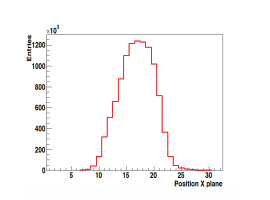
\includegraphics[width=1.1\textwidth]{03_GraphicFiles/chapter6_BeamTests/Nice_May2018/profileX.png}
\caption{Horizontal plane.}
\label{chap6::fig::May_HodoprofX}
\end{subfigure}
\begin{subfigure}[t]{.5\textwidth}
\centering
\includegraphics[width=1.1\textwidth]{03_GraphicFiles/chapter6_BeamTests/Nice_May2018/profileY.png}	
\caption{Vertical plane.}
\label{chap6::fig::May_HodoprofY}
\end{subfigure}
\caption{Mono-dimensional spatial profiles of the beam recorded by the hodoscope.}
\label{chap6::fig::May_Hodoprof1D}
\end{figure}

The spatial performance of the hodoscope are also determined by the number of fibers involved in each interaction. This parameter has been studied and the results are shown in \figurename~\ref{chap6::fig::May_HodoClusters} for the two axes. As expected, in most of the interactions one single fiber per axis is involved. However, a significant amount of events shows two or more fibers involved in at least one of the two axes. Moreover, since the acquisition was performed in hodoscope AND mode, at least one fiber per axis should be mandatory to validate the event and send it to the \gls{utca} for the acquisition. This behavior reveals a problem, probably in the \gls{fe} board firmware, which is discussed in section~\ref{chap6::subsec::mayDiscussion}. 
 
\begin{figure}
\begin{subfigure}[t]{.5\textwidth}
\centering
\includegraphics[width=1.\textwidth]{03_GraphicFiles/chapter6_BeamTests/Nice_May2018/clusterX.png}
\caption{Horizontal plane.}
\label{chap6::fig::May_HodoClusX}
\end{subfigure}
\begin{subfigure}[t]{.5\textwidth}
\centering
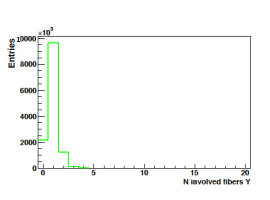
\includegraphics[width=1.\textwidth]{03_GraphicFiles/chapter6_BeamTests/Nice_May2018/clusterY.png}	
\caption{Vertical plane.}
\label{chap6::fig::May_HodoClusY}
\end{subfigure}
\caption{Number of involved fibers per event recorded by the hodoscope for the two planes.}
\label{chap6::fig::May_HodoClusters}
\end{figure}

The objective of the hodoscope is to obtain information about the beam for what concerns the direction and precise timing of each incident ion (or incident bunch, at high beam intensity). The timing performance has been also analyzed with this low beam intensity run. The absolute time (with repsect to the board internal clock), is measured separately for the two fiber planes and for the trigger signal. Concerning the fiber plane time, it corresponds to the arrival time of the first event detected in the defined time coincidence window. The coincidence window was fixed, for this test, to 3 board internal clock counts, corresponding to 24~ns. To be noticed that the time measurement features implemented on the \gls{fe} board was still under development at the moment of testing, and the trigger arrival time was measured according to the internal board clock. A dedicated clock with 250~ps resolution was already implemented for the hodoscope fiber time measurements on both planes. The installation of a dedicated \gls{tdc} on the card for the trigger channel is foreseen for the final configuration, fort which the \gls{tof} between the absorber and the hodoscope interactions will be measured. Given the problem detected in the previous analysis stage, which determines the presence of events with no coincidence between the two planes, the timing performance analysis is limited to coincidence events, selected at the analysis stage.
\figurename~\ref{chap6::fig::May_HodoDeltaT} shows the distributions of the measured time for the two separate fiber planes (x - left and y - right). The distributions \gls{fwhm} is 6.8~ns and 5.3~ns for the x ans y plane, respectively. The verified performance are worse with respect to the expected values, but improvements in the time calculation in the \gls{fe} board are still needed to achieve the design setup. 

\begin{figure}
\begin{subfigure}[t]{.5\textwidth}
\centering
\includegraphics[width=1.1\textwidth, trim={0 0.6cm 0 0} , clip=true]{03_GraphicFiles/chapter6_BeamTests/Nice_May2018/TX-Ttrig.png}
\caption{Horizontal plane.}
\label{chap6::fig::May_HododTx}
\end{subfigure}
\begin{subfigure}[t]{.5\textwidth}
\centering
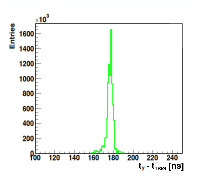
\includegraphics[width=1.1\textwidth]{03_GraphicFiles/chapter6_BeamTests/Nice_May2018/TY-Ttrig.png}	
\caption{Vertical plane.}
\label{chap6::fig::May_HododTy}
\end{subfigure}
\caption{Distribution of the time difference between the trigger arrival time and the time measured by the two hodoscope fiber planes.}
\label{chap6::fig::May_HodoDeltaT}
\end{figure}

The distribution of the measured absolute time difference between the two fiber planes has also been studied and is reported in \figurename~\ref{chap6::fig::May_HodoDeltaTFibers}. The distribution is expected to be centered in $t_{x}-t_{y} = 0$, and its width is expected to reflect the hodoscope time resolution, given the superior resolution of the reference clock (250~ps). The experimental distribution has a mean value of 2.4~ns and a width \gls{fwhm} of 3.5~ns.

\begin{figure}[!htbp]
\centering
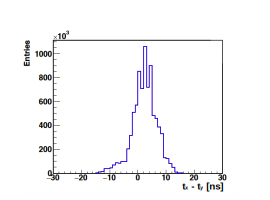
\includegraphics[width=0.75\textwidth]{03_GraphicFiles/chapter6_BeamTests/Nice_May2018/TX-TY.png}
\caption{Distribution of the time difference between the two hodoscope fiber planes for x-y coincidence events.}
\label{chap6::fig::May_HodoDeltaTFibers}
\end{figure}

As mentioned, the hodoscope detection efficiency has been tested for increasing beam intensity, reported here as external trigger detection rate. As previously highlighted, even if in AND configuration the hodoscope is supposed to record only x-y coincidence events, single plane events are also recorded. For this reason, both the single plane and coincidence event detection efficiency are reported in \figurename~\ref{chap6::fig::May_HodoEffInt} as a function of the trigger rate for the two working mode of the hodoscope (AND and OR) triggered by the external signal provided by the coincidence of the two scintillators on beam. 

\begin{figure}[!htbp]
\centering
\includegraphics[width=0.7\textwidth]{03_GraphicFiles/chapter6_BeamTests/Nice_May2018/MAY_Eff_intensity.png}
\caption{Hodoscope detection efficiency as a function of the trigger detected rate for the different acquisition modes. The solid lines corresponds to acquisitions with the hodoscope in AND configuration, the dashed lines to the OR configuration. Red curves represent events in x-y plane coincidence, while blue curves includes single plane and coincidence events.}
\label{chap6::fig::May_HodoEffInt}
\end{figure}

The detection efficiency levels shown in the plot in \figurename~\ref{chap6::fig::May_HodoEffInt} are lower than the expected: the hodoscope is expected to provide a coincidence efficiency beyod 90~\%. The expected detection efficiency has been obtained only in OR configuration and including both single plane and coincidence events. Moreover, acquisition problems have been verified at high trigger rate in hodoscope OR configuration, so that the data point at 280~kHz is missing. These results are discussed in section~\ref{chap6::subsec::mayDiscussion}. 

\subsection{Discussion}\label{chap6::subsec::mayDiscussion} 

After a preliminary test performed in December 2017 in order to first test the final acquisition system on beam, in May 2018 the 32$\times$32 scintillating fiber hodoscope has been tested on beam for the first time with the final \gls{utca}-based acquisition system. The promising results presented in the previous section allowed to estimate the hodoscope performance, highlight the main issues for what concerns the detector, the \gls{fe} and read-out boards and the acquisition system, and plan the development advancements.
In particular, it has been shown that:
\begin{itemize}
\item the hodoscope spatial response it satisfactory and the beam profile has been correctly recorded;
\item in most of the events, 1 or 2 fibers per detection plane are involved;
\item the time response is limited to a 6-7~ns time window with a non-optimized system;
\item a detection efficiency beyond 90\% can be achieved at low beam intensity.
\end{itemize}

Notwithstanding the encouraging results, the \gls{fe} board and acquisition firmware and software showed some issues during this first test. In particular, the working AND mode showed an unexpected behavior. With this working mode, only events with time coincidence between the horizontal and the vertical fiber planes should be recorded, but also non-coincidence events has been collected. Some laboratory tests have been performed after the end of the beam test campaign, and a possible explanation has been found in the data processing at the hodoscope \gls{fe} board level. The analog signals emerging from the hodoscope read-out \glspl{pm} are collected on the board and converted to logic with the application of a fixed threshold. The logic signal time width depends on the time-over-threshold of the analog signal, so that low amplitude analog signals can trigger the acquisition but result in very short logic output. If the AND function implemented on the board to verify the coincidence takes more time than the logic signal width, the coincidence can be triggered but the logic signal related to the hit fiber can be lost. 
This effect could explain the presence of single plane interaction also in AND working mode. In addition, this effect could also be the cause of the very low efficiency in AND configuration (below 60\%) shown in figure~\ref{chap6::fig::May_HodoEffInt}.
The presented timing performance have been obtained with a preliminary time calculation method. In particular, a dedicated clock was already implemented on the \gls{fe} board for the hodoscope fiber time measurement, but the arrival time of the external trigger signal was measured according to the general card clock at low resolution. This measurement method affected the time resolution which is below the expectations. Also the distribution of the time difference between the fibers in the two detection planes measured in coincidence shows a width of 3.5~ns \gls{fwhm}, and a mean value of 2.4~ns, while no time difference is expected between the two fiber planes and a 1~ns resolution is the requirement for this detector. This not satisfactory performance are probably due to the time measurement method, which selects the first event in the time coincidence window as time reference. In case of background contamination, un-correlated background events collected in the coincidence window degrades the time resolution. 

The aforementioned issues are expected to be solved by the planned improvements to the firmware of the hodoscope \gls{fe} boards, as well as by a fine tuning of the working parameters. A gain and a threshold are indeed fixed on the hodoscope board \gls{asic} for each read-out channel (each fiber), and an appropriate calibration of their values will probably allow to obtain analog signals with sufficient amplitude to result in larger logic signal, able to trigger the coincidence read-out and be transferred to the data acquisition with non-zero values. This should improve the overall efficiency of the system and guarantee the correct functionality of the AND acquisition setting. Moreover, the proper threshold should reduce the background contamination, thus improving the timing performance. 
An automatic calibration method has been developed in the summer 2018 in collaboration with an internship student, and applied to characterize the hodoscope board \gls{asic} behavior for background measurements. The same strategy will be applied during a dedicated beam test before the end of 2018 to define the hodoscope optimal working parameters for the monitoring of proton beams. A second dedicated test will be then necessary for the characterization of the hodoscope with carbon ions, which are expected to induce different response due to an increased energy deposit in the scintillating fibers.
     
Finally, before the end of this first test, the \gls{utca} trigger capabilities have been tested with two hodoscope cards to mimic the coupling of two camera components. This first attempt allowed to create the bases for the firmware and electronics development of the following months, which aimed to prepare the system for the first test of a multi-collimated camera configuration, i.e. the couling of hodoscope and absorber, performed in September 2018 and described in section~\ref{chap6::sec::september2018}. 
\newpage

\section{Collimated camera: September 2018}\label{chap6::sec::september2018}

\subsection{Experimental results}\label{chap6::subsec::mayResults} 

\subsection{Discussion}\label{chap6::subsec::mayDiscussion} 

\clearpage
%\printbibliography[heading=subbibintoc]
